\begin{figure}[H]
    \begin{subfigure}{0.3\textwidth}
        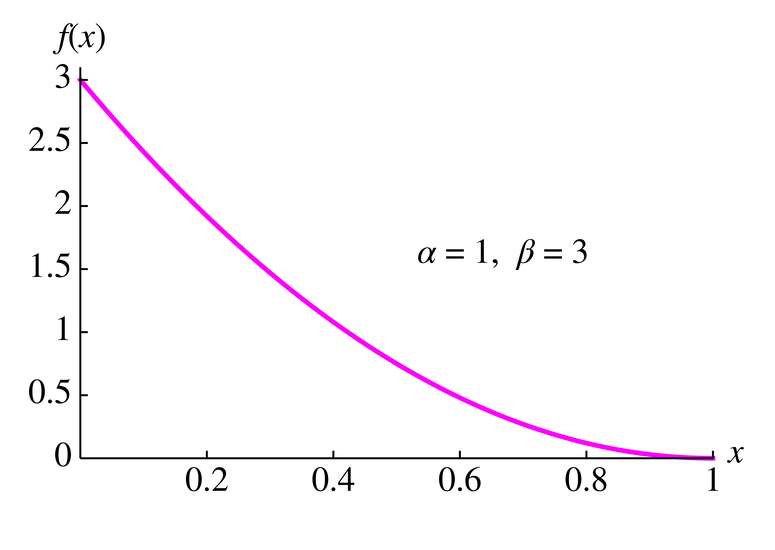
\includegraphics[width=1\linewidth]{beta.png}
        \caption{beta}
    \end{subfigure}
    \begin{subfigure}{0.3\textwidth}
        \includegraphics[width=1\linewidth]{binominal.png}
        \caption{binominal}
    \end{subfigure}
    \begin{subfigure}{0.3\textwidth}
        \includegraphics[width=1\linewidth]{epsilon_lambda.png}
        \caption{epsilon lambda}
    \end{subfigure}
\end{figure}

\begin{figure}[H]
    \begin{subfigure}{0.3\textwidth}
        \includegraphics[width=1\linewidth]{gama.png}
        \caption{gama}
    \end{subfigure}
    \begin{subfigure}{0.3\textwidth}
        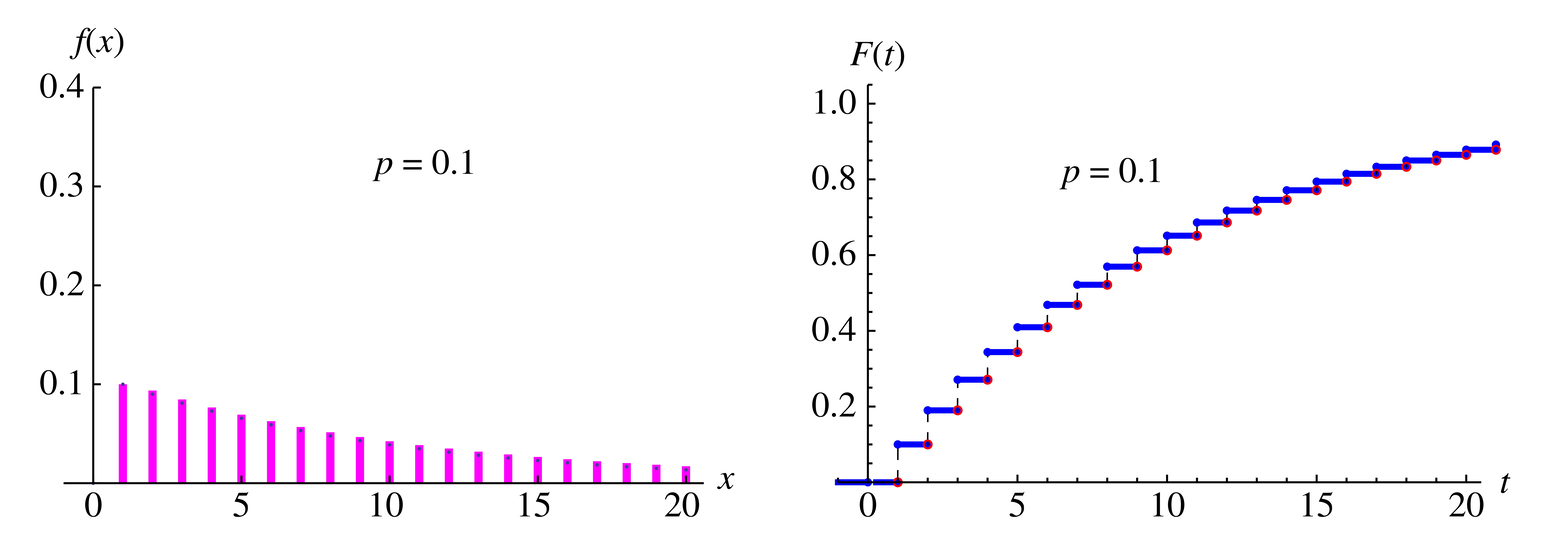
\includegraphics[width=1\linewidth]{geom.png}
        \caption{geom}
    \end{subfigure}
    \begin{subfigure}{0.3\textwidth}
        \includegraphics[width=1\linewidth]{hyperg.png}
        \caption{hyperg}
    \end{subfigure}
\end{figure}

\begin{figure}[H]
    \begin{subfigure}{0.3\textwidth}
        \includegraphics[width=1\linewidth]{normal.png}
        \caption{normal}
    \end{subfigure}
    \begin{subfigure}{0.3\textwidth}
        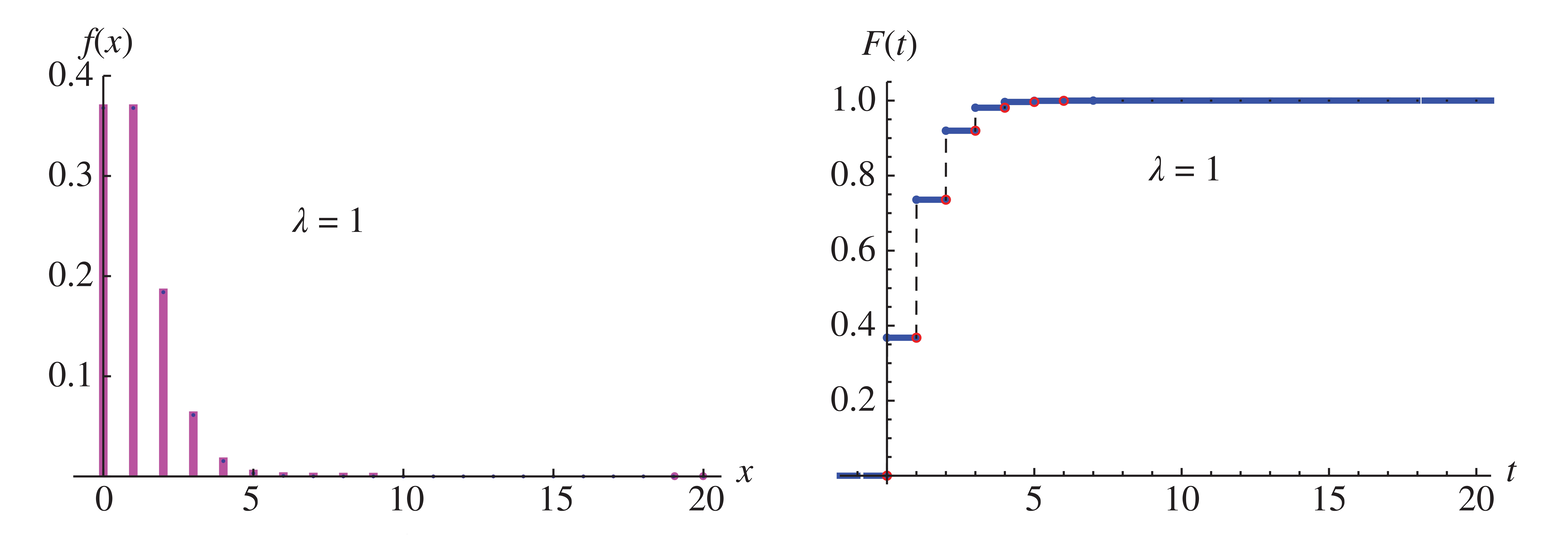
\includegraphics[width=1\linewidth]{poisson.png}
        \caption{poisson}
    \end{subfigure}
    \begin{subfigure}{0.3\textwidth}
        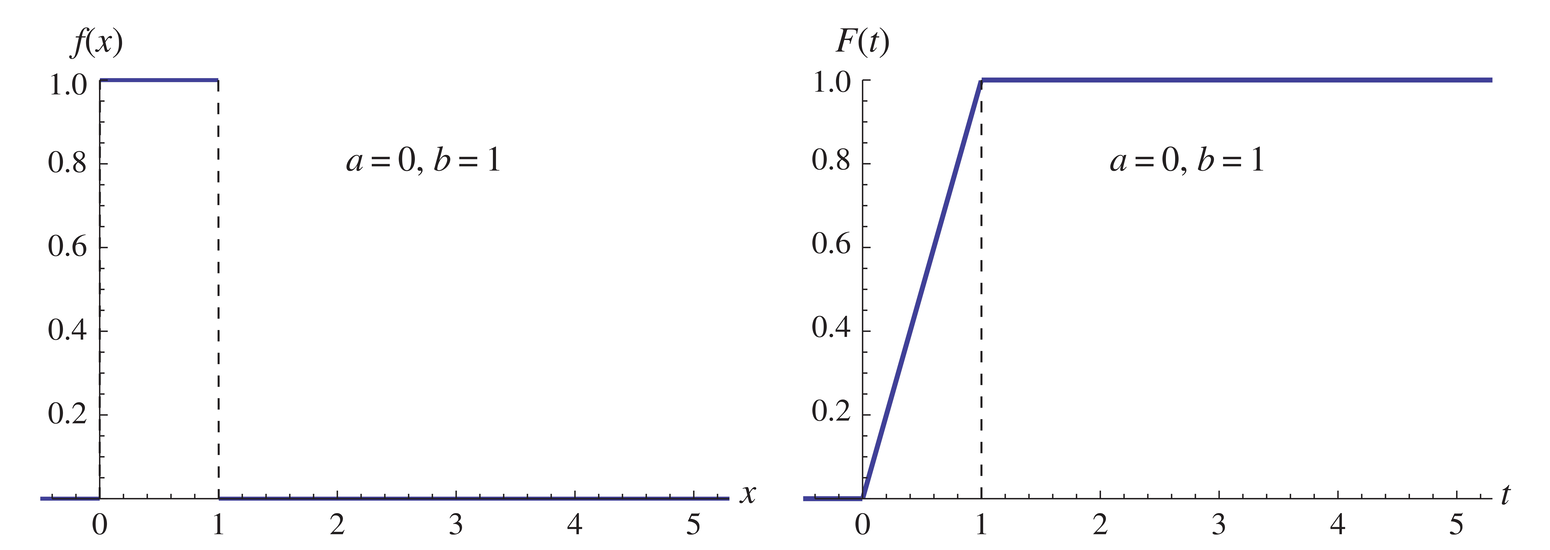
\includegraphics[width=1\linewidth]{uniforme.png}
        \caption{uniforme}
    \end{subfigure}
\end{figure}